\chapter{Datasets}
\label{chap:datasets} 

In this chapter I introduce the datasets annotated using the tool described in chapter~\ref{chap:design}, describe a little background around each one and examine some statistics. It is left to chapter~\ref{chap:annotation} to  analyse the annotation process used to create these datasets and evaluate the annotation process.

\section{Datasets}

The datasets comprise a mix of relatively small scale image sets annotated for the sake of evaluating and developing the annotation method, image sets as test cases for future projects and a particular niche which seems suited to this kind of annotation method which is counting wildlife. In each case annotation time was between around an hour to around eight hours for the largest.

The sizes of objects in these datasets in general are small compared to more mainstream object detection datasets. This can be seen in figure~\ref{fig:box_sizes}, where compared to the Pascal VOC \cite{Everingham2008}, or COCO \cite{Lin2014}, the box sizes are smaller compared to the image size and less widely distributed. 

Figure \ref{fig:box_sizes_plot}  shows the object sizes (in pixels) of all the datasets together for comparison. In particular, the \emph{aerial penguin} and \emph{scott base} datasets have particularly tiny objects (not shown on the figure in order to preserve the scale). It can be seen that although the box sizes are relatively small in terms of the relative size to the image that at full resolution the objects can be relatively large in pixels.

Two different types of annotations are used in the annotations of these datasets. Circular annotations are used for very small objects and for counting objects where precise localisation is of less concern; circular annotations are also used for apples where it just happens to match the object shape well. The difference to the object detector is little, instead of estimating two parameters, width and height it is simply a radius. In all other respects a circle is treated as a square for computations such as \gls{IOU} overlap.

\begin{figure}[ht]
\centering
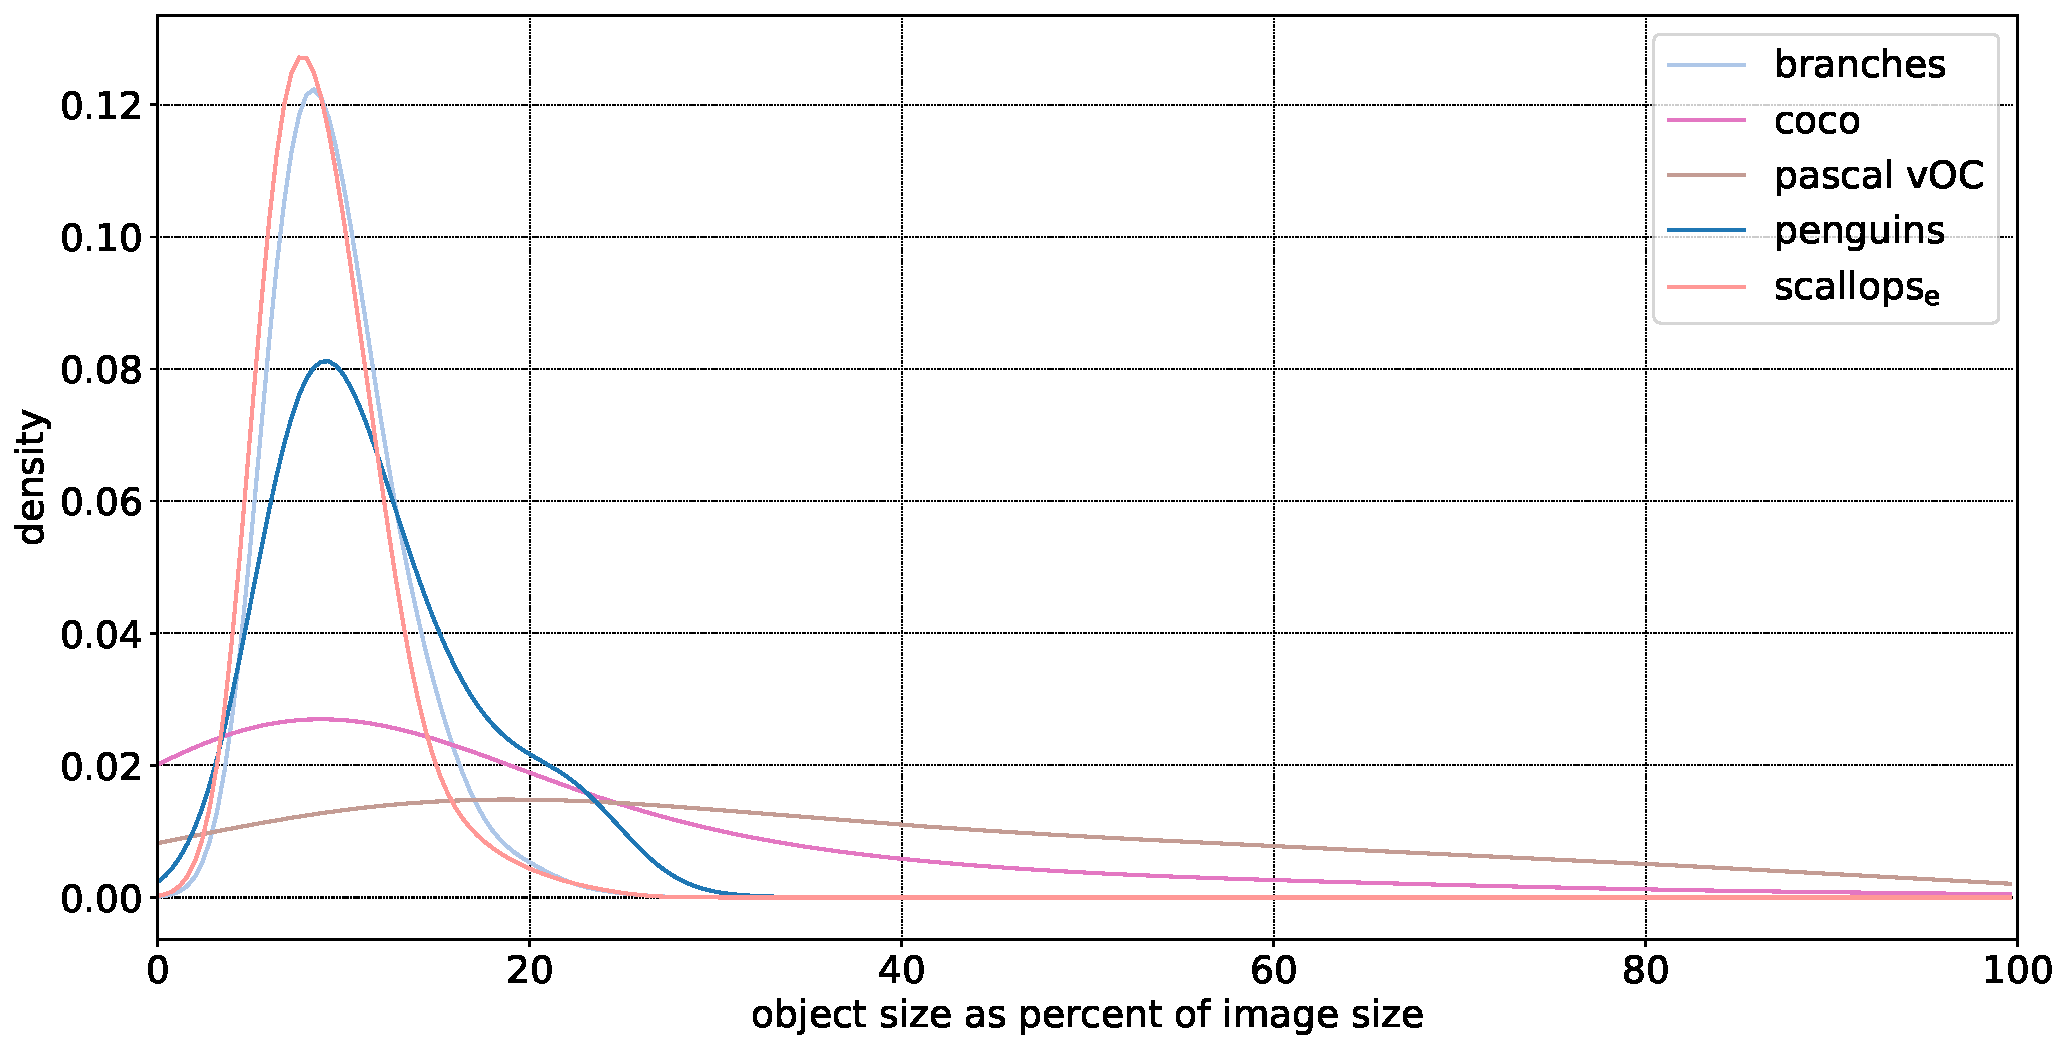
\includegraphics[width=1.0\linewidth]{charts/summaries/sizes_density.pdf}
\caption{Object bounding box size distributions as percent object to image size (average of width and height ratios) }
\label{fig:box_sizes}
\end{figure}


\begin{figure}[ht]
\centering
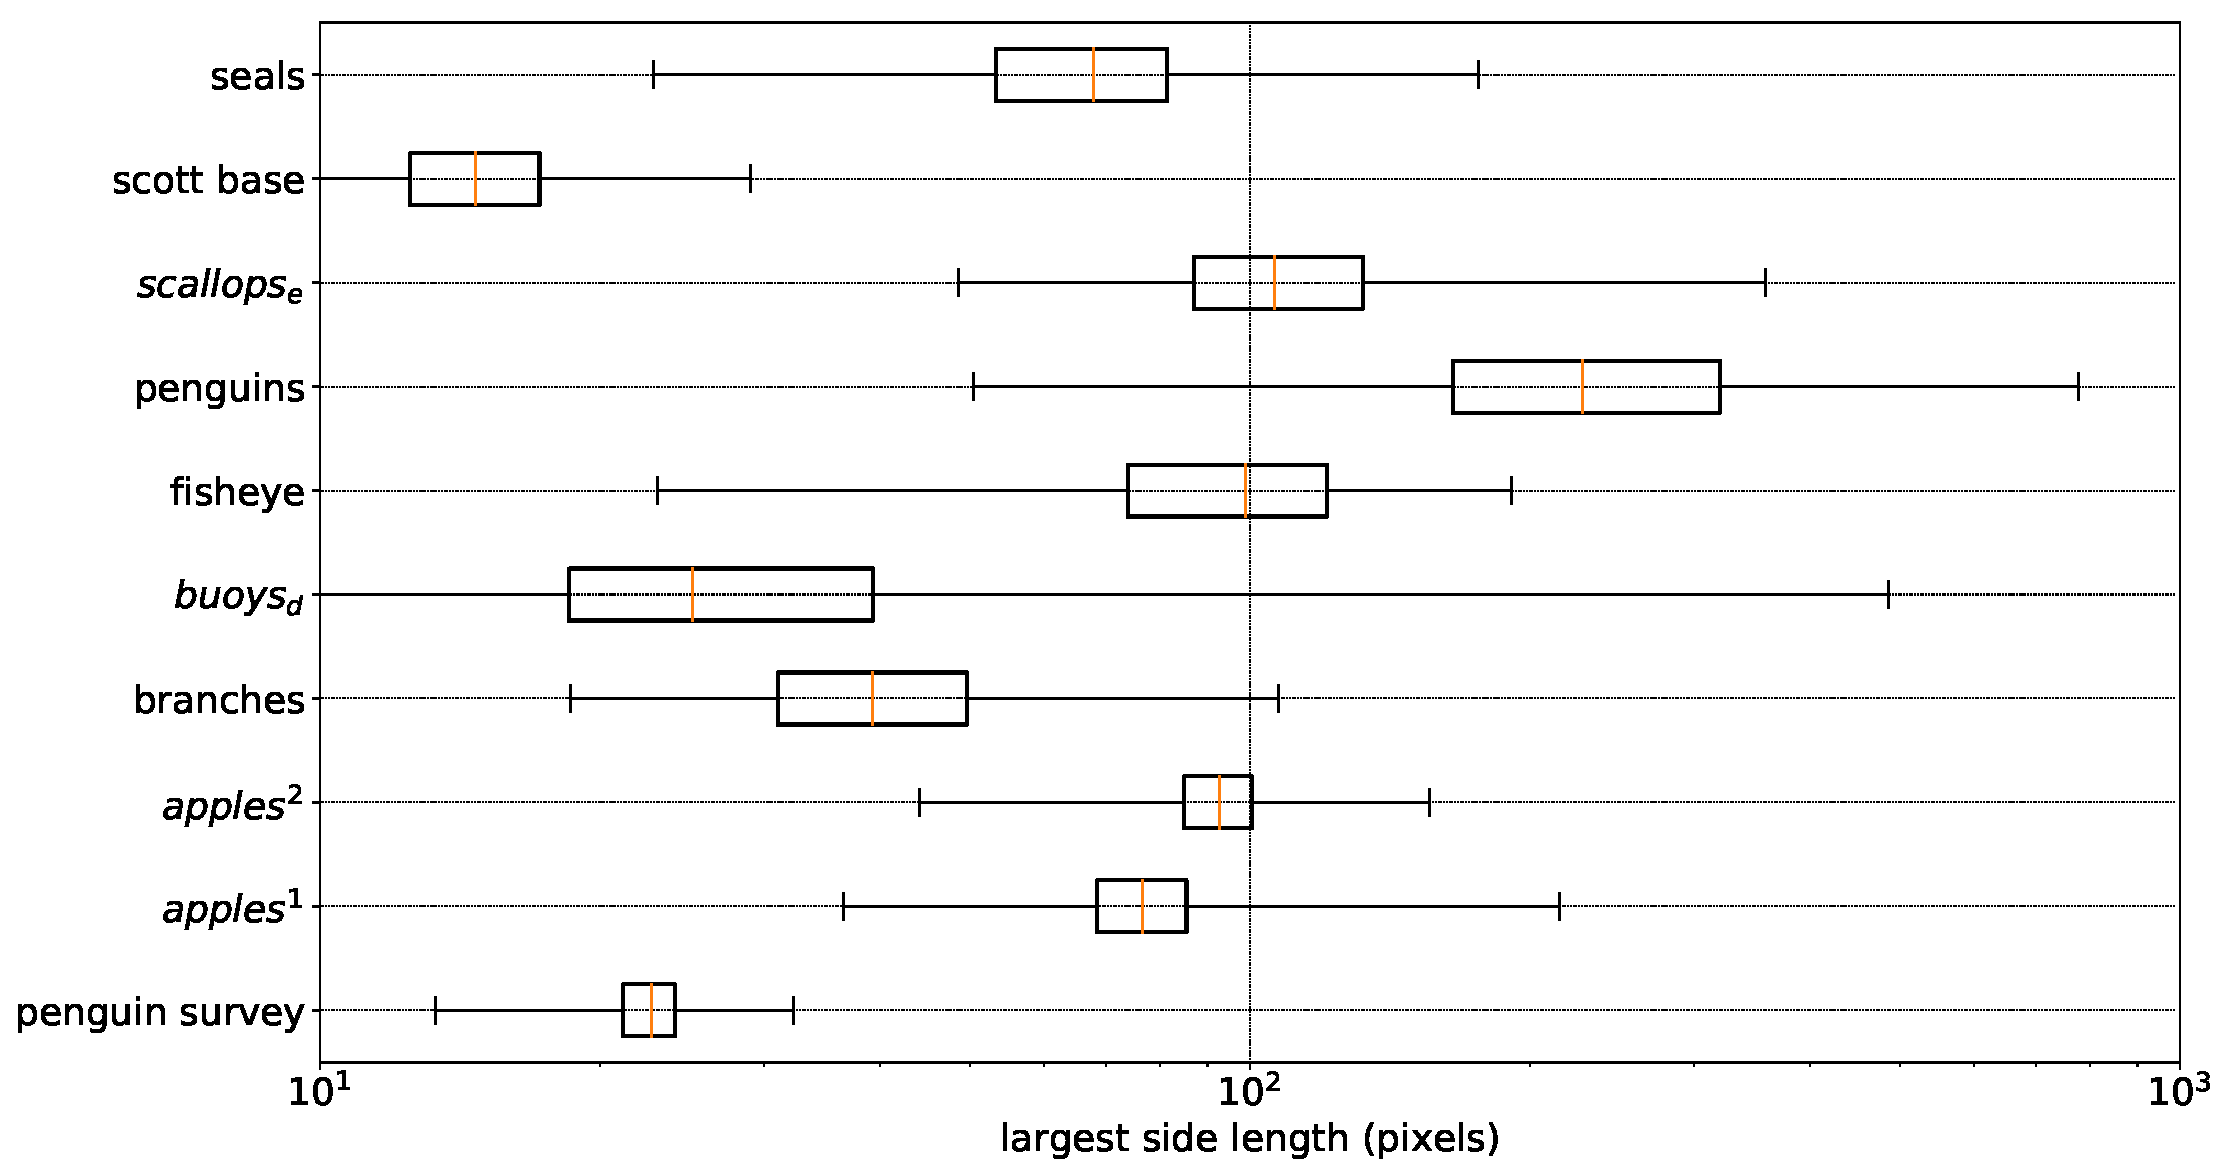
\includegraphics[width=1.0\linewidth]{charts/summaries/sizes_boxplot.pdf}
\caption{ Sizes in pixels of boxes for all annotated datasets }
\label{fig:box_sizes_plot}
\end{figure}





\section{Development}

One dataset 

\begin{figure*}[h!]
\centering
\begin{subfigure}[t]{1.0\linewidth}
  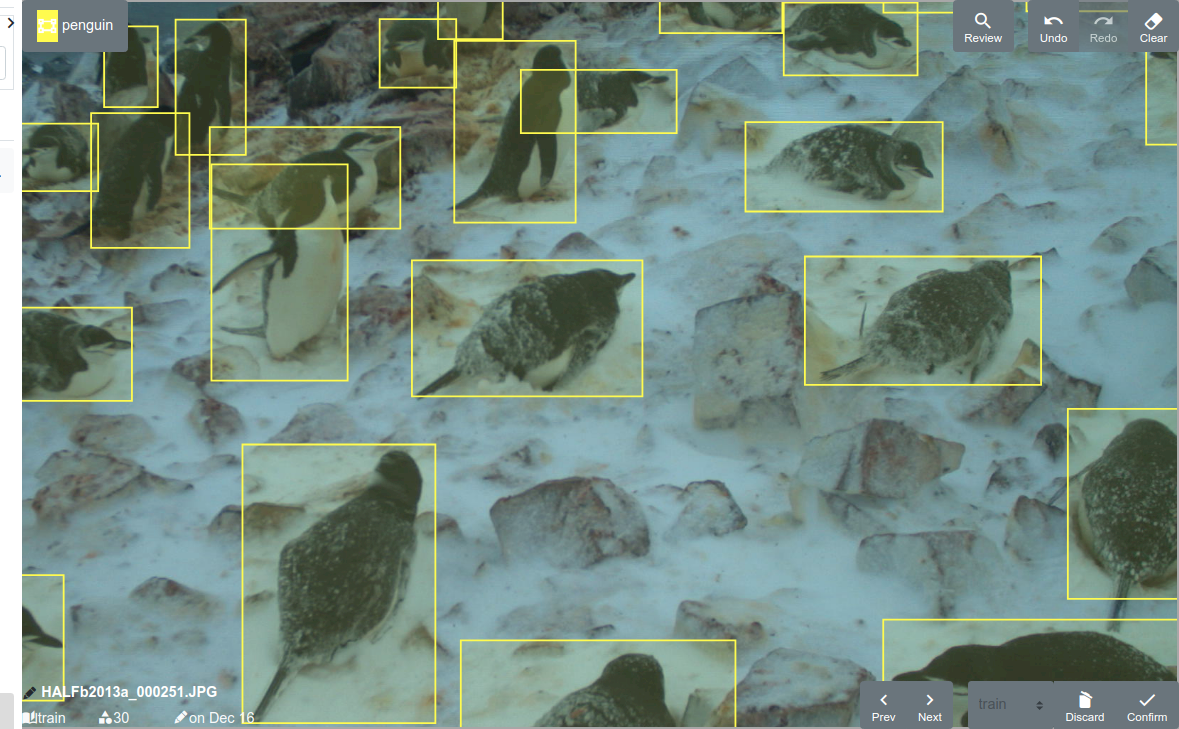
\includegraphics[width=0.475\linewidth]{figures/annotation/screenshots/penguins.png}
  \hfill
  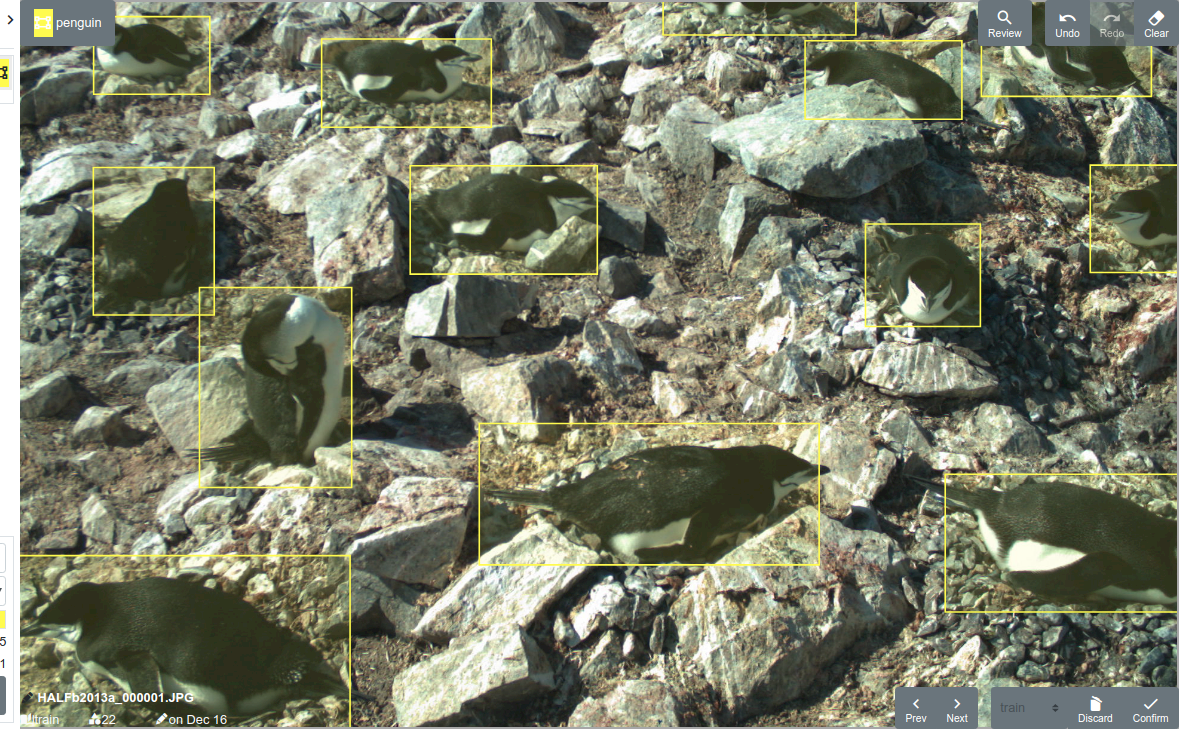
\includegraphics[width=0.475\linewidth]{figures/annotation/screenshots/penguins2.png}
  \caption{}
\end{subfigure}

\begin{subfigure}[t]{1.0\linewidth}
  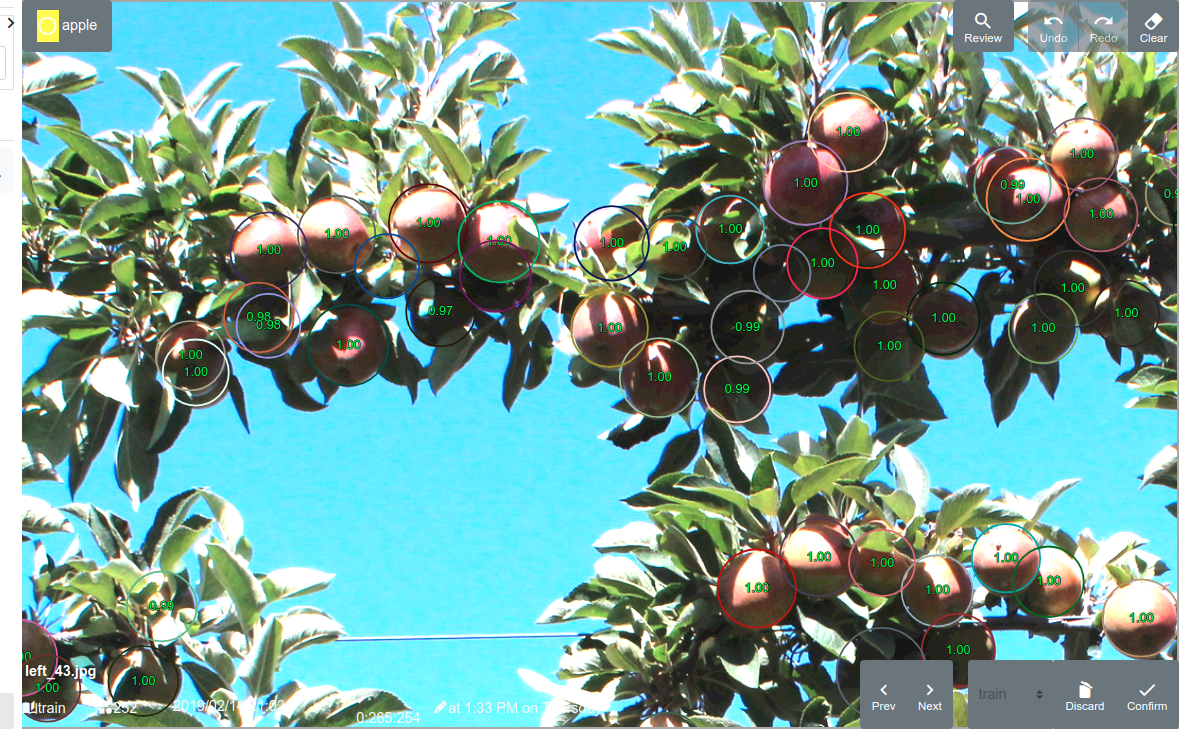
\includegraphics[width=0.475\linewidth]{figures/annotation/screenshots/apples_big.png}
  \hfill
  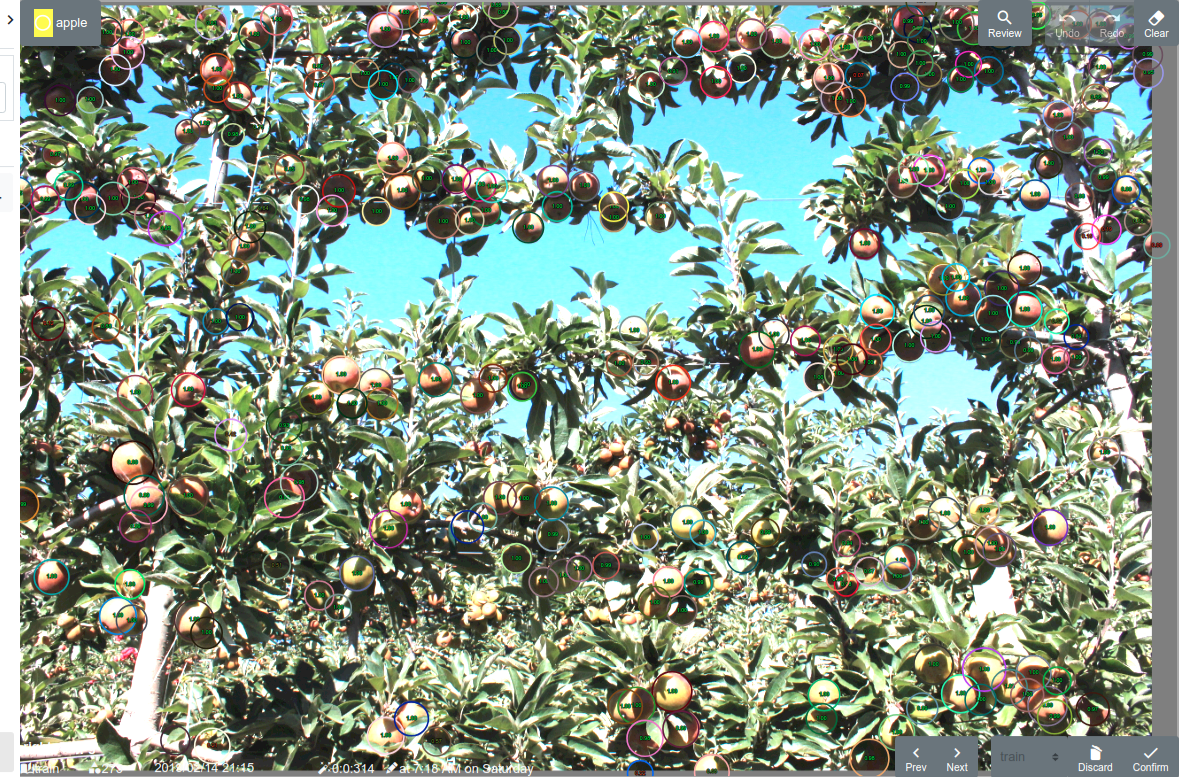
\includegraphics[width=0.475\linewidth]{figures/annotation/screenshots/apples_small.png}
  \caption{}
\end{subfigure}


\begin{subfigure}[t]{1.0\linewidth}
  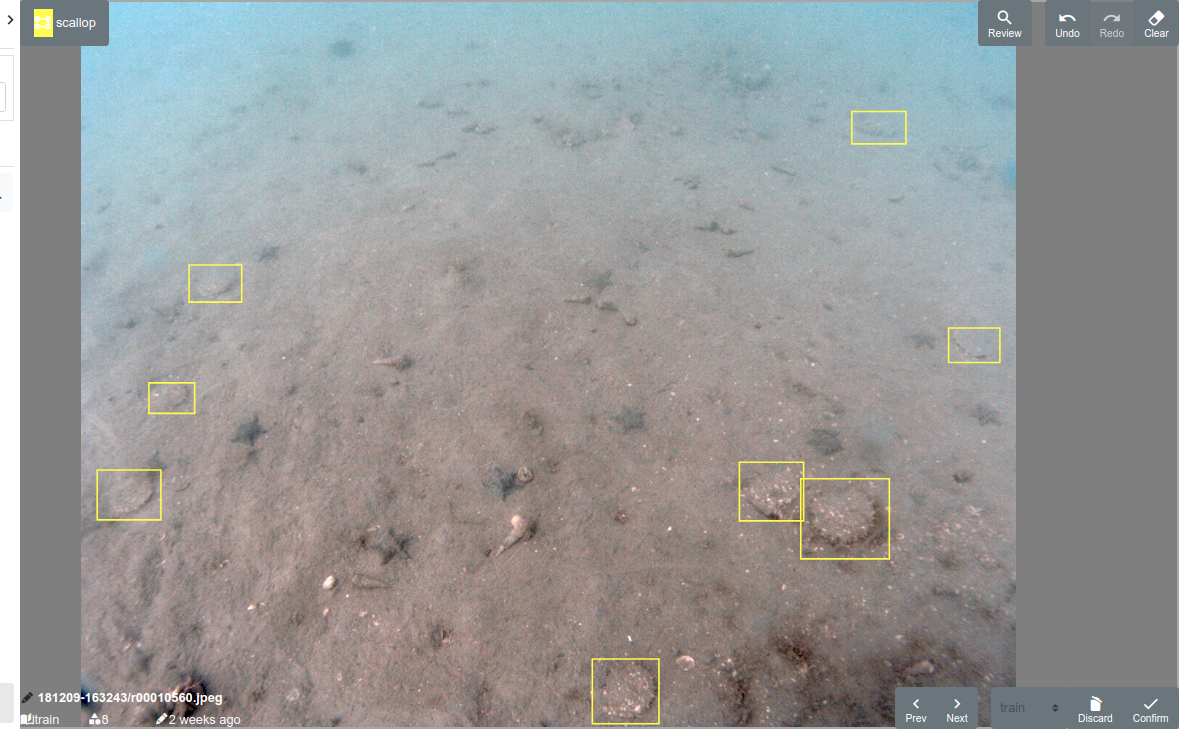
\includegraphics[width=0.475\linewidth]{figures/annotation/screenshots/scallops.png}
  \hfill
  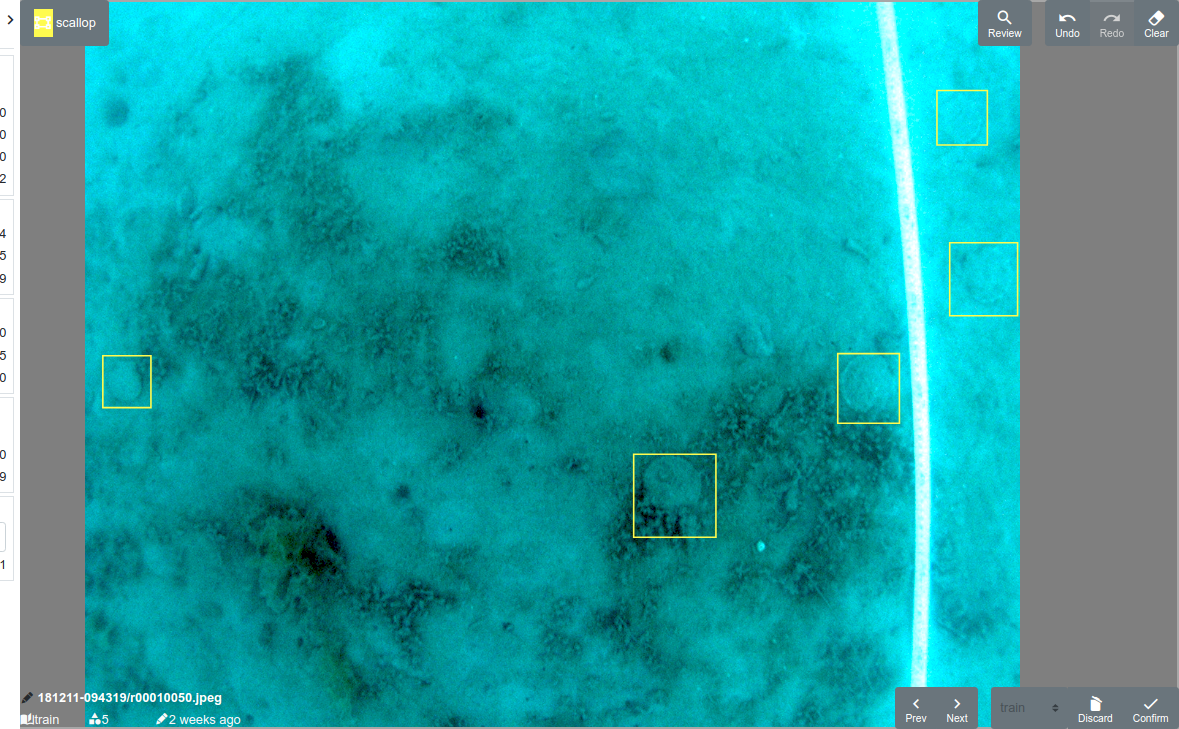
\includegraphics[width=0.475\linewidth]{figures/annotation/screenshots/scallops3.png}
  \caption{}

\end{subfigure}

\caption{ }
\label {fig:apple_examples}
\end{figure*}






\begin{figure*}[h!]
\centering

\begin{subfigure}[t]{0.5\textwidth}
  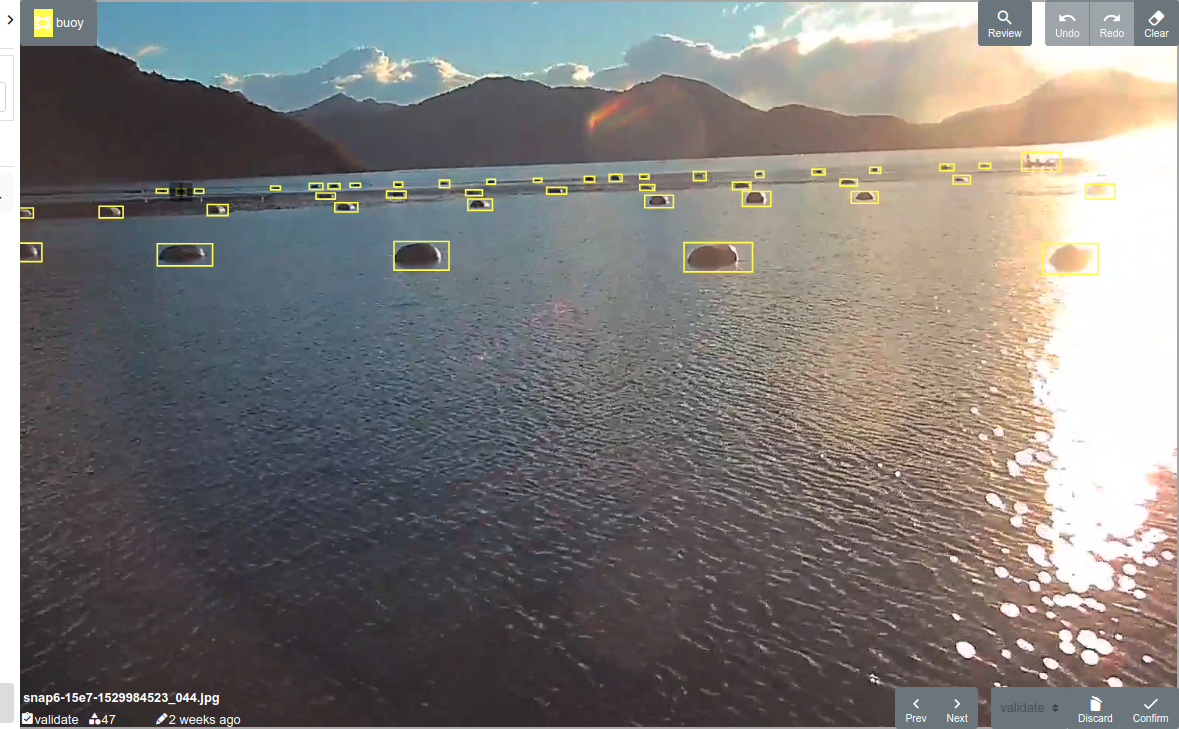
\includegraphics[width=0.95\textwidth]{figures/annotation/screenshots/buoys.png}
  \caption{}
\end{subfigure}%
\begin{subfigure}[t]{0.5\textwidth}
  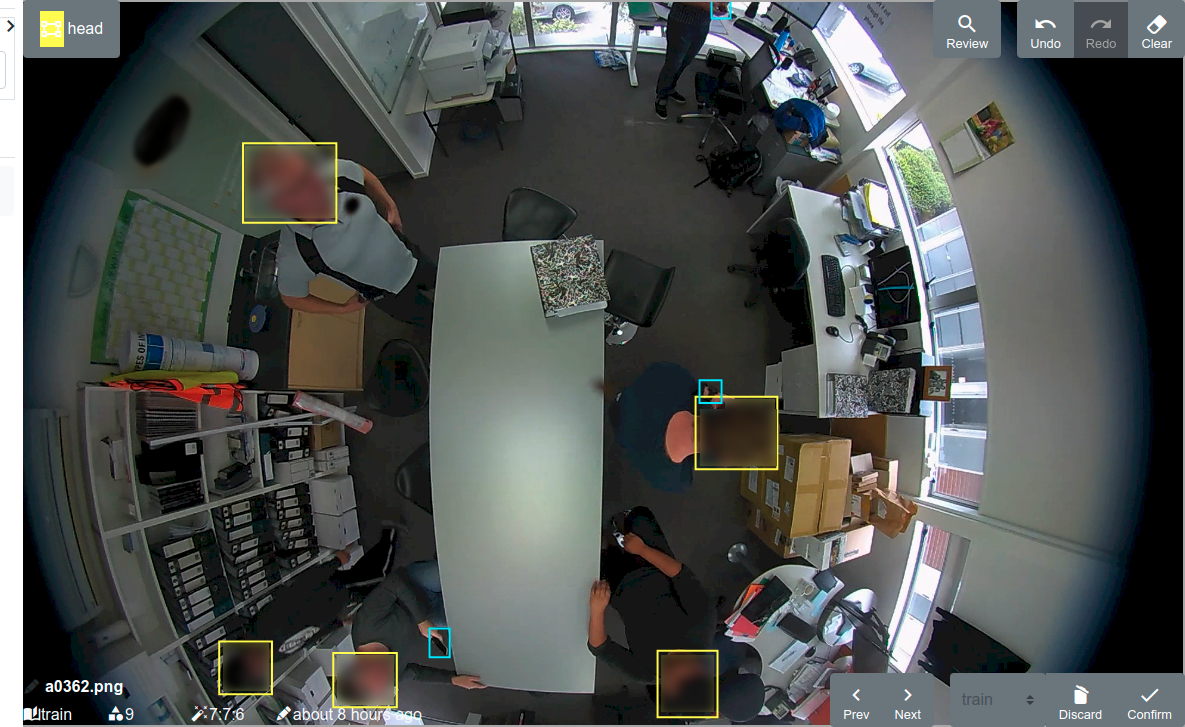
\includegraphics[width=0.95\textwidth]{figures/annotation/screenshots/victor.png}
  \caption{fisheye: Fish-eye head and cellphone detection }
\end{subfigure}

\begin{subfigure}[t]{0.5\textwidth}
  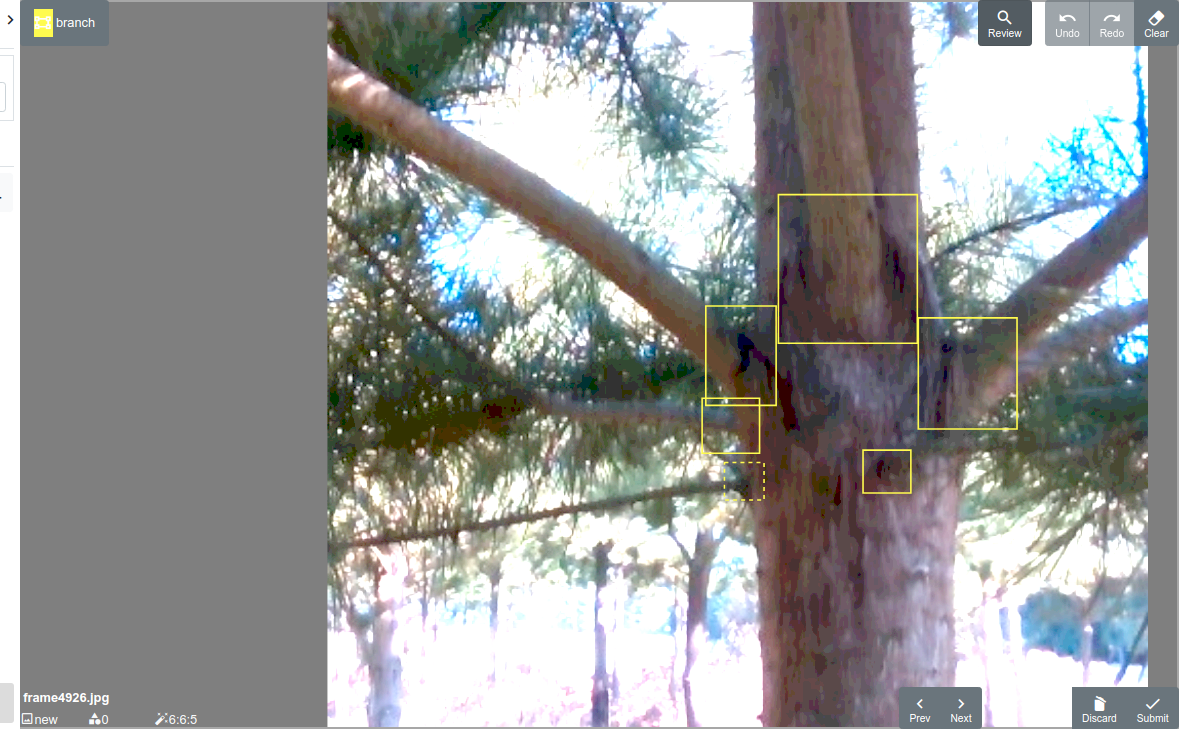
\includegraphics[width=0.95\textwidth]{figures/annotation/screenshots/branches3.png}
  \caption{branches: Tree branch intersection detection}
\end{subfigure}%
\begin{subfigure}[t]{0.5\textwidth}
  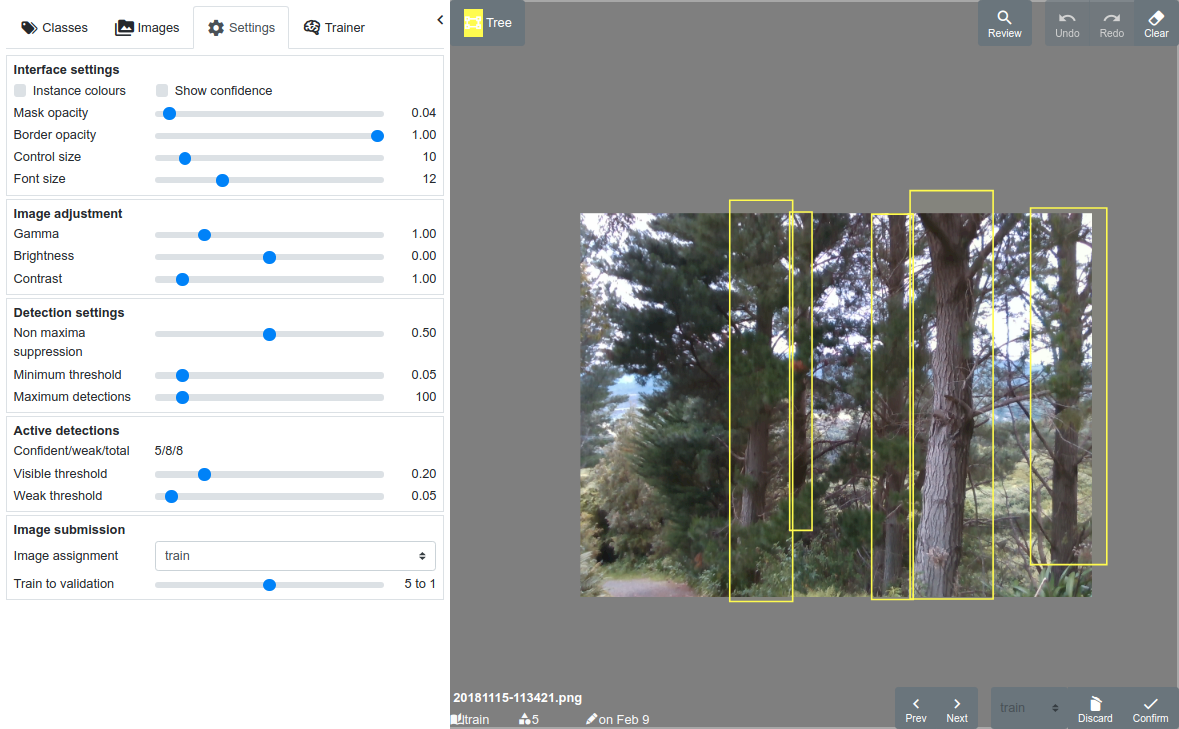
\includegraphics[width=0.95\textwidth]{figures/annotation/screenshots/josh_trees.png}
  \caption{}
\end{subfigure}

\caption{ }
\label {fig:dataset_images}
\end{figure*}